\section{Oblak točaka}

Oblak točaka je skupina podataka koji definiraju neki objekt u prostoru. Oblak točaka se obično generira pomoću trodimenzionalnog skenera. Oblaci točaka imaju veliku primjenu u rekonstrukcijama predmeta, vizualizaciji, animaciji, virtualnoj i proširenoj stvarnosti te industrijskoj proizvodnji i kontroli kvalitete. U trodimenzionalnome kartezijevom sustavu svaka točka je definirana s tri atributa, a to su njene x, y i z koordinate. Uz te osnovne podatke svaka točka također može sadržavati i podatke o njenoj boji.

\begin{figure}[h!]
  \centering
  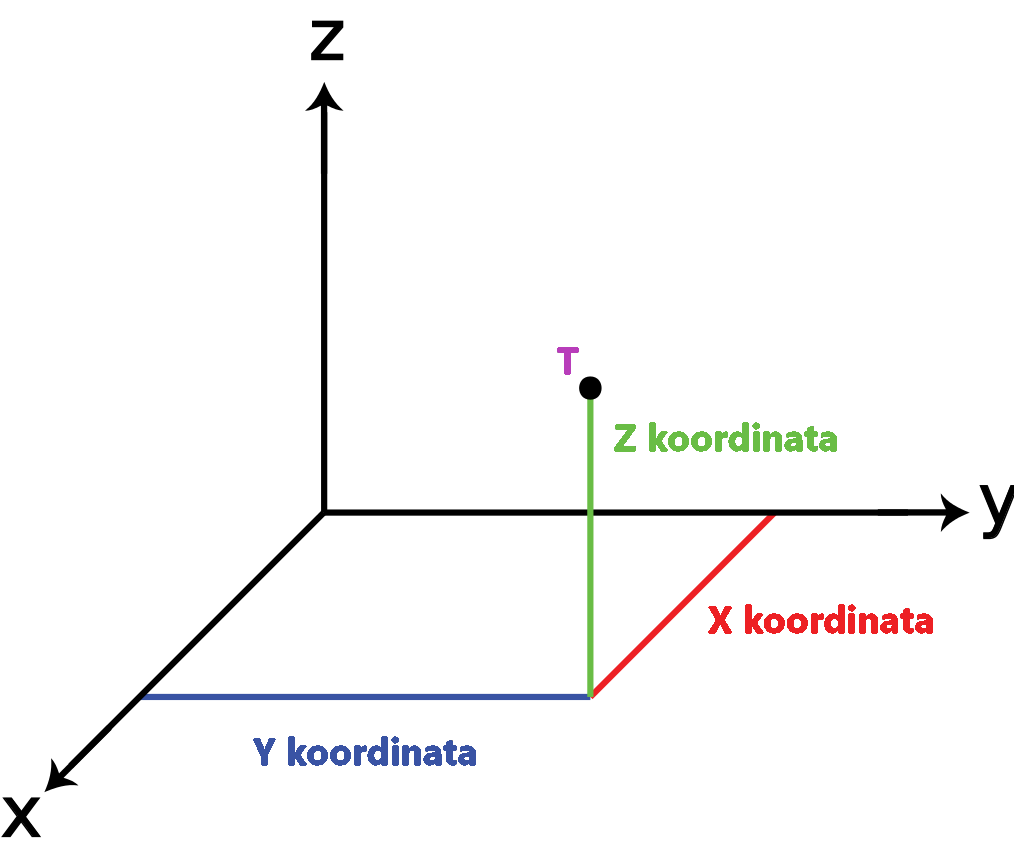
\includegraphics[scale=0.3]{images/point-coordinates.png}
  \caption{Ilustracija točke u kartezijevom koordinatnome prostoru}
  \label{fig:point_coordinates}
\end{figure}

\begin{figure}[h!]
  \centering
  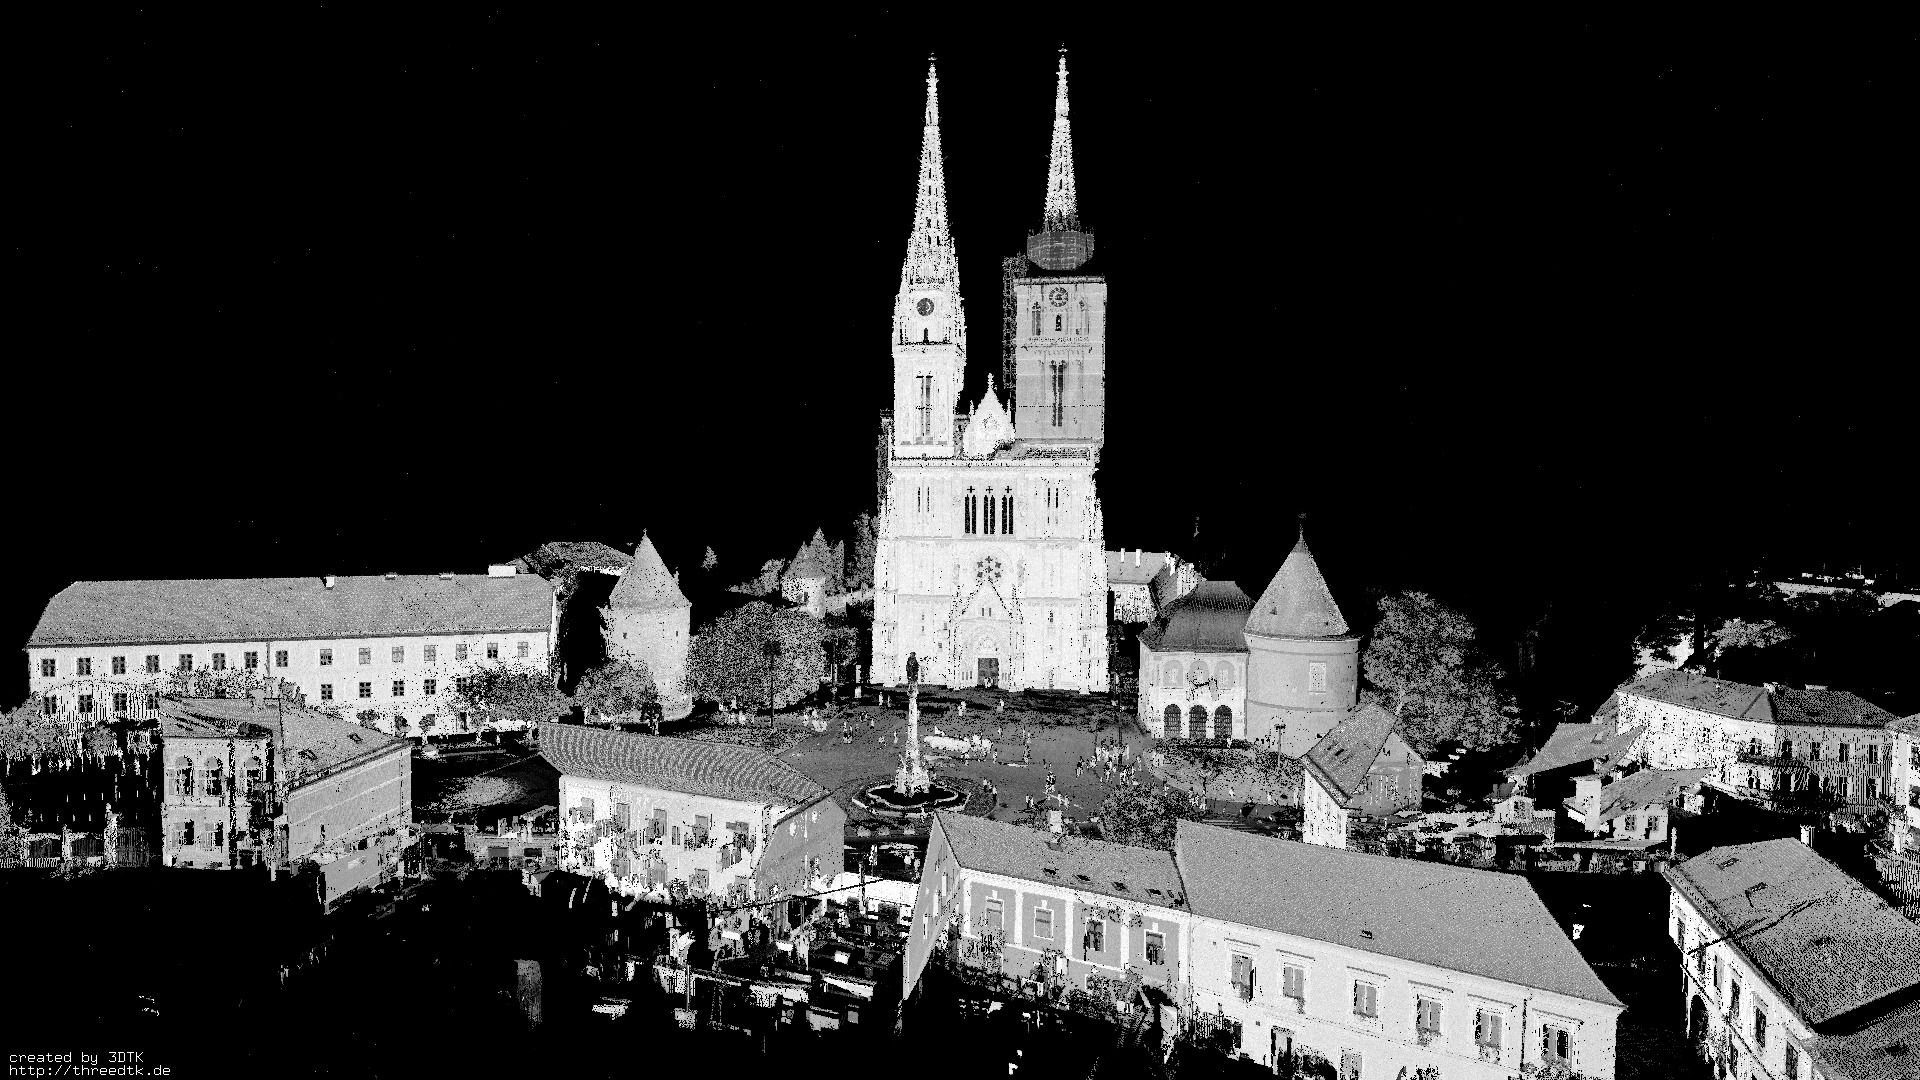
\includegraphics[scale=0.2]{images/katedrala-point-cloud.jpg}
  \caption{Oblak točaka katedrale u Zagrebu\cite{cloud:katedrala}}
  \label{fig:point_cloud_exmaple}
\end{figure}

Na slici \ref{fig:point_cloud_exmaple} se vidi skup točaka koji opisuje katedralu u Zagrebu te okolne objekte. Skup se sastoji od oko 22 milijuna točaka. Skup točaka je mnogo jednostavnije koristiti za mapiranje objekata od slika zato što se lakše može obraditi na računalu. Ti podaci su zapravo spremljeni u tekstualne datoteke pa su lako prenosivi i čitljivi. Konkretno metode u ovome radu koriste oblak točaka prikupljen s rotirajućim laserima na vozilu. Jedan taj skup točaka predstavlja stanje okoline vozila u jednome vremenskome trenutku.